\documentclass[conference]{IEEEtran}
\IEEEoverridecommandlockouts
% The preceding line is only needed to identify funding in the first footnote. If that is unneeded, please comment it out.
\usepackage[numbers,sort]{natbib}
\usepackage{amsmath,amssymb,amsfonts}
\usepackage{algorithmic}
\usepackage{graphicx}
\usepackage{textcomp}
\usepackage{xcolor}
\usepackage{tikz}
\usetikzlibrary{arrows.meta,positioning,shapes.geometric}
\def\BibTeX{{\rm B\kern-.05em{\sc i\kern-.025em b}\kern-.08em
    T\kern-.1667em\lower.7ex\hbox{E}\kern-.125emX}}
\begin{document}

\title{BT-CAP: An Agentic Bio-Reasoning Framework and LightGBM Ranker for Nominating Glioma Synaptic and Immune Targets
\\}

\author{\IEEEauthorblockN{Eric Yang}
\IEEEauthorblockA{\textit{Department of Electrical \& Computer Engineering} \\
\textit{Rice University}}
\and
\IEEEauthorblockN{Jasper Chen}
\IEEEauthorblockA{\textit{Department of Electrical \& Computer Engineering} \\
\textit{Rice University}}
}

\maketitle

\begin{abstract}
Single-cell RNA sequencing reveals critical cellular heterogeneity in brain tumors, yet identifying functional synaptic drivers and T-cell immune synapse targets in gliomas remains hindered by high-expression metabolic noise and standard LLM hallucinations. To overcome this, we present BT-CAP (Brain Tumor Cell Annotation Platform), an agentic bio-reasoning framework and machine learning ranker. BT-CAP anchors Gemini 2.5 Flash reasoning with deterministic in-house table-lookup tools, eliminating hallucinated interactions across multi-step queries. To rank targets across a 9,580-gene universe, we integrate 32-dimensional scETM gene embeddings extracted from 20,000+ single cells into a Positive-Unlabeled LightGBM model. Augmented with scETM co-expression vectors, BT-CAP achieves 0.742 AUROC for tumor synaptic genes and 0.725 AUROC for immune synapse genes, significantly outperforming standard table-rule baselines (0.631 AUROC). The framework filters background metabolic noise and surfaces auditable candidates, including NCL, BSG, MPZL1, and GPR37L1, which are deployed directly within an interactive web portal.
\end{abstract}

\begin{IEEEkeywords}
Single-cell RNA sequencing (scRNA-seq), Transformer-based models, Cell type annotation, Brain tumor heterogeneity, Tumor microenvironment
\end{IEEEkeywords}

\section{Introduction}
Single-cell RNA sequencing (scRNA-seq) has revolutionized our understanding of cellular heterogeneity in brain tumors like gliomas and medulloblastomas. However, existing frameworks—such as Azimuth and scANVI—often struggle to annotate malignant states because they rely on non-malignant reference cells and are susceptible to technical "dropout" noise \cite{CHAUHAN2025100371}. To bridge this gap, we present BT-CAP (Brain Tumor Cell Annotation Platform). By leveraging transformer-based foundation models like Geneformer \cite{theodoris2023transfer} and TOSICA \cite{chen2023transformer}, BT-CAP utilizes self-attention mechanisms to capture complex gene regulatory networks in a context-aware manner, outperforming traditional linear models \cite{szalata2024transformers}. By integrating automated annotation, scalable vector storage, and interactive visualization, BT-CAP provides a robust, clinical-grade portal for rapid and reproducible neuro-oncology analysis.

\section{Methodology}

\subsection{System Architecture and Agentic RAG Flow}
To overcome output-truncation and hallucination limits of unanchored Large Language Models (LLMs) processing single-cell data, we built an agentic Retrieval-Augmented Generation (RAG) framework anchored to structured in-house datasets. The architecture constrains LLM generation to verified tabular evidence (Figure~\ref{fig:system_architecture}).

\subsubsection{Query Routing and Tool Tracing}
An intent-based Router dispatches incoming biological queries ($Q$) across specialized Python lookup tools:
\begin{itemize}
    \item \textbf{CellChat Lookup (\texttt{cellchat\_lookup}):} Queries 922 significant ligand-receptor edges re-analyzed across electrophysiologically (Ephys) stratified tumor and immune clusters.
    \item \textbf{Differential Expression (\texttt{deg\_lookup}):} Extracts within-cluster DEGs ($\log_2\text{FC}$, adjusted $p$-value, percent expression) stratified by cell type and IDH status.
    \item \textbf{Dataset Stats (\texttt{count\_lookup}):} Checks cluster cell counts, enforcing $N \ge 10$ cells per side to eliminate small-sample noise.
    \item \textbf{Pathway Contrast (\texttt{exclusive\_pathway\_lookup}):} Identifies pathways exclusively enriched in specific functional Ephys states.
\end{itemize}

\begin{figure*}[t]
\centering
\resizebox{0.98\textwidth}{!}{%
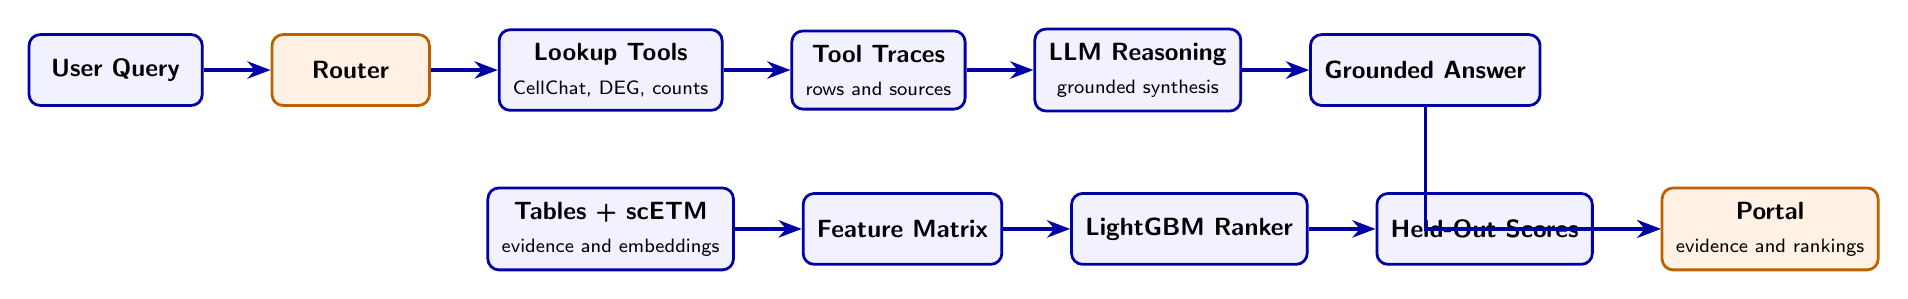
\begin{tikzpicture}[
    node distance=0.75cm and 0.85cm,
    base/.style={
        draw=blue!65!black,
        fill=blue!5,
        rounded corners=4pt,
        line width=1pt,
        align=center,
        inner sep=5pt,
        font=\sffamily\small,
        text=black,
        minimum height=0.9cm,
        minimum width=2.2cm
    },
    router/.style={
        base,
        draw=orange!75!black,
        fill=orange!10,
        minimum width=2cm
    },
    arrow/.style={
        -Stealth,
        draw=blue!65!black,
        line width=1.2pt
    }
]

% Grounded question-answering lane
\node (query) [base] {\textbf{User Query}};
\node (router) [router, right=of query] {\textbf{Router}};
\node (tools) [base, right=of router] {\textbf{Lookup Tools}\\[1pt]
    \scriptsize CellChat, DEG, counts};
\node (traces) [base, right=of tools] {\textbf{Tool Traces}\\[1pt]
    \scriptsize rows and sources};
\node (llm) [base, right=of traces] {\textbf{LLM Reasoning}\\[1pt]
    \scriptsize grounded synthesis};
\node (answer) [base, right=of llm] {\textbf{Grounded Answer}};

% Gene-ranking lane
\node (data) [base, below=0.95cm of tools] {\textbf{Tables + scETM}\\[1pt]
    \scriptsize evidence and embeddings};
\node (features) [base, right=of data] {\textbf{Feature Matrix}};
\node (ranker) [base, right=of features] {\textbf{LightGBM Ranker}};
\node (scores) [base, right=of ranker] {\textbf{Held-Out Scores}};
\node (portal) [router, right=of scores] {\textbf{Portal}\\[1pt]
    \scriptsize evidence and rankings};

\draw [arrow] (query) -- (router);
\draw [arrow] (router) -- (tools);
\draw [arrow] (tools) -- (traces);
\draw [arrow] (traces) -- (llm);
\draw [arrow] (llm) -- (answer);
\draw [arrow] (data) -- (features);
\draw [arrow] (features) -- (ranker);
\draw [arrow] (ranker) -- (scores);
\draw [arrow] (scores) -- (portal);
\draw [arrow] (answer) |- (portal);

\end{tikzpicture}%
}
\caption{BT-CAP system architecture. Natural-language questions are routed to deterministic lookup tools, and the resulting traces constrain LLM synthesis. In parallel, structured evidence and scETM embeddings feed the LightGBM ranker. The portal exposes both grounded answers and held-out gene scores without placing the ranker downstream of the LLM.}
\label{fig:system_architecture}
\end{figure*}

Empty query results log explicit absence of evidence rather than generating synthetic entries, guaranteeing zero hallucinated interactions or DEGs.

\subsubsection{Reasoning Backend Selection}
Tool traces are passed into the LLM reasoning layer. Benchmarking revealed that MedGemma 1.5-4B truncated output on 37.5\% (9/24) of multi-step test queries. Conversely, Gemini 2.5 Flash reliably parsed traces with 100\% (24/24) accuracy, providing cited observation-versus-interpretation answers without hallucination. Gemini 2.5 Flash was thus selected as the primary reasoning engine.

\subsection{scETM Gene Embedding Extraction}
To capture latent gene co-expression networks obscured by high fold-change noise, we integrated a single-cell Embedded Topic Model (scETM) pipeline.

\subsubsection{Preprocessing and Model Training}
From an in-house dataset of 254,777 glioma cells (\texttt{adata.h5ad}), we sampled a cell-type-stratified corpus of 20,381 cells across 12 lineages (max 1,800 cells/type; 20,126 genes) and batch-corrected across 25 patient samples. scETM was trained with a 32-dimensional embedding space ($K=32$) and 50 biological topics ($T=50$) using variational inference (batch size 2,000; 1,000 epochs). We extracted the dense gene embedding matrix $\boldsymbol{\rho} \in \mathbb{R}^{20,126 \times 32}$.

\subsubsection{Embedding Feature Engineering}
Two feature sets were generated for downstream ranking:
\begin{itemize}
    \item \textbf{Level 1 (\texttt{emb\_0--emb\_31}):} Direct 32-D latent vectors ($\boldsymbol{\rho}$).
    \item \textbf{Level 2 (\texttt{knn\_frac\_synaptic}, \texttt{knn\_frac\_immune}):} Fold-safe $k$-NN ($k=20$) neighborhood density features calculating the proportion of a gene's 20 nearest neighbors that belong to the ground-truth label sets.
\end{itemize}

\subsection{LightGBM Positive-Unlabeled (PU) Gene Ranker}
We constructed a Positive-Unlabeled (PU) LightGBM model to rank targets across a genome-wide scale without penalizing unannotated genes as false negatives.

\subsubsection{Feature Space and Ground-Truth Labels}
Rankings are evaluated at the \textbf{Gene $\times$ Cell Type $\times$ IDH Context} level (27,346 rows across 9,580 genes; 42 features). Features encompass CellChat probabilities, DEG metrics, cell counts, 32-D scETM vectors, and fold-safe $k$-NN densities. Models are supervised using SynGO 1.3 (1,789 genes for $p_{\text{tumor\_synaptic}}$) and QuickGO GO:0001772 (244 genes for $p_{\text{immune\_synapse}}$).

\subsubsection{Validation Scheme}
To prevent data leakage, we implemented a 5-fold StratifiedGroupKFold grouped strictly by \textbf{Gene} across 5 random seeds. Held-out genes were evaluated out-of-fold using AUROC, AUPRC, and Precision@10 metrics.

\subsection{Portal Integration and Evidence Delivery}
The reasoning agent and gene ranker were integrated into the BT-CAP portal as a read-only layer over the analytical outputs. The backend loads the RAG engine, CellChat and DEG tables, held-out LightGBM scores, and scETM embeddings once, then exposes endpoints for grounded questions, gene-level evidence, filtered rankings, and nearest-neighbor retrieval. No biological score or interaction is calculated in the browser.

A dedicated \textbf{Genes} workspace displays table-only and table-plus-scETM scores across cell-type and IDH contexts, together with functional badges, top features, CellChat edges, DEG rows, and scETM neighbors. The portal and \texttt{nominate\_lookup} use the same score loader, preventing disagreement between gene cards and chat responses. Each answer includes structured tool traces, while unsupported questions return an explicit absence of evidence. An automated regression suite compared portal and command-line retrieval, reference-gene scores, and cached MedGemma responses.
\section{Results}

\subsection{Deterministic RAG Retrieval and Reasoning Benchmark}
Evaluating the agentic bio-reasoning framework across 24 multi-step biological queries ($Q_{9}$--$Q_{32}$) confirmed that constraining LLM generation with deterministic table-lookup tools achieves 100\% (24/24) required term retrieval while eliminating hallucinations. Across all queries, the tool-calling pipeline retrieved exact CellChat edges, DEGs, and cell counts without introducing fake ligand-receptor pairs or false expression metrics.

In model comparison tests, Gemini 2.5 Flash significantly outperformed MedGemma 1.5-4B. MedGemma suffered from reasoning loops and truncated outputs on 37.5\% (9/24) of test questions (e.g., $Q_{9}, Q_{10}, Q_{26}$). In contrast, Gemini 2.5 Flash successfully synthesized verified tool traces into cited, structured answers separating direct observations from biological interpretations with zero hallucinations.

\subsection{Quantitative Target Ranking Performance}
The Positive-Unlabeled (PU) LightGBM model was evaluated out-of-fold across 27,346 rows (9,580 unique genes) using 5-fold \texttt{StratifiedGroupKFold} CV grouped by gene. As shown in Table~\ref{tab:model_performance}, augmenting tabular features with 32-dimensional scETM co-expression embeddings provided a consistent performance boost across both target arms.

\begin{table}[t]
\centering
\caption{Out-of-Fold Model Performance Comparison}
\label{tab:model_performance}
\small
\begin{tabular}{lccc}
\hline
\textbf{Model Arm} & \textbf{AUROC} & \textbf{AUPRC} & \textbf{P@10} \\ \hline
\textit{Baselines} & & & \\
DEG $|\log_2\text{FC}|$ Baseline & 0.612 & 0.188 & 0.200 \\
3-Table Heuristic Rule & 0.631 & 0.226 & 0.000 \\ \hline
\textit{Tumor Synaptic Arm} & & & \\
Tables Only & 0.675 & 0.332 & 0.800 \\
\textbf{Tables + scETM Embeddings} & \textbf{0.742} & \textbf{0.437} & \textbf{0.900} \\
scETM Embeddings Only & 0.738 & 0.433 & 0.900 \\ \hline
\textit{Immune Synapse Arm} & & & \\
Tables Only & 0.666 & 0.015 & 0.100 \\
\textbf{Tables + scETM Embeddings} & \textbf{0.725} & \textbf{0.021} & \textbf{0.300} \\
scETM Embeddings Only & 0.706 & 0.020 & 0.200 \\ \hline
\end{tabular}
\end{table}

For the \textbf{Tumor Synaptic Arm}, combining tabular features with scETM vectors achieved 0.742 AUROC and 0.437 AUPRC, markedly outperforming single-table heuristic rules (0.631 AUROC). For the \textbf{Immune Synapse Arm}, adding scETM embeddings increased AUROC from 0.666 to 0.725, shifting top predicted ranks away from myeloid expression noise toward true T-cell synapse drivers.

\subsection{Portal Deployment and Cross-Interface Validation}
Portal and command-line retrieval agreed on tool selection, required evidence, and deterministic answer text for \textbf{44/44 benchmark questions}. Scores and context ranks also matched \texttt{nominate\_lookup} for all 33 literature-reference genes. Thirty-two genes had model scores, while the unscored gene \emph{AXL} correctly remained absent rather than receiving an artificial zero. MedGemma produced \textbf{24/24 cache hits} with zero provider calls and no cache modification.

The interface exposes these guarantees as auditable evidence. For example, an \emph{NRXN1} gene card shows program probabilities, the features driving its score, CellChat and DEG rows, minimum group size, and held-out fold. Because the ranked list, gene card, neighbor view, and grounded chat read the same artifacts, each nomination remains linked to its biological context and source evidence. Figure~\ref{fig:portal_gene_card} demonstrates how a ranked gene is connected to its cell-type context, model score, and supporting evidence within the portal.

\begin{figure*}[!t]
    \centering
    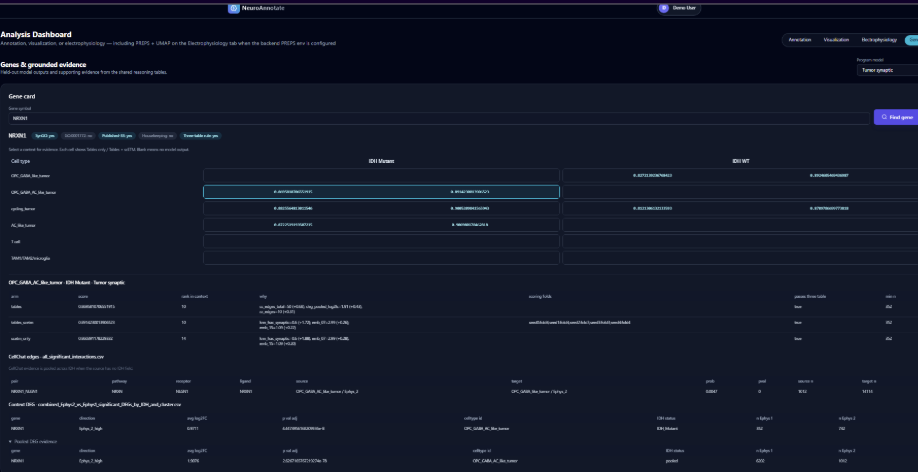
\includegraphics[width=0.98\textwidth]{figures/portal_card.png}
    \caption{Evidence-linked nomination of \emph{NRXN1} in the integrated BT-CAP portal. The gene card displays context-specific tumor-synaptic and immune-synapse predictions together with their driving features, CellChat interactions, differential-expression evidence, cell-count support, and held-out scoring information.}
    \label{fig:portal_gene_card}
\end{figure*}

\subsection{Metabolic Noise Filtering and Gene Nominations}
A critical failure of traditional fold-change and table-only ranking is the inflation of high-expression metabolic background noise (mitochondrial, ferritin, and off-target genes). Integrating scETM embeddings effectively resolved this bias:
\begin{itemize}
    \item \textbf{Housekeeping Correction:} Under table-only ranking, 19 of the top 100 hits were off-list mitochondrial and ferritin noise. With scETM features integrated, 78 of 83 top housekeeping hits were correctly identified as functional ribosomal genes explicitly annotated within SynGO.
    \item \textbf{Tumor Synaptic Candidates:} The model retained known reference targets (\emph{GRIA2, NRXN1, PTPRZ1, GRIK2}) and ranked \emph{GPR37L1, COL9A1, NCL, ITGB8}, and \emph{PSAP} among the leading filtered novel nominees.
    \item \textbf{Immune Synapse Candidates:} The model retained known T-cell and MHC-II markers, including \emph{CD28, HLA-DRA}, and \emph{CD74}, while ranking \emph{HLA-DQB1, PILRA, TNFRSF1B, PTPRC}, and \emph{CD69} among the leading filtered novel nominees.
\end{itemize}
All predicted probabilities and ranker feature contributions were integrated directly into the web portal frontend for auditable target inspection.


\section{Discussion}

The combined results support a layered target-nomination strategy: deterministic retrieval defines the evidence boundary, scETM embeddings add functional context, and the portal exposes both the prediction and its provenance. The system should therefore be interpreted as a hypothesis-generation framework rather than an autonomous source of experimental conclusions.

\subsection{Limitations and Technical Challenges}

The positive labels remain incomplete: genes absent from SynGO or GO:0001772 are unlabeled, not confirmed negatives. This limitation is most apparent in the immune arm, where the model reached 0.725 AUROC but only 0.021 AUPRC. In addition, the analysis uses one in-house glioma dataset and depends on predicted Ephys classes, IDH labels, and available cell counts. CellChat, DEG, and embedding associations therefore do not establish causal signaling or therapeutic efficacy.

The fixed question benchmark cannot represent every possible query, and cached MedGemma answers test reproducible delivery rather than new-generation stability. Gemini also introduces cost, latency, and data-governance concerns. Technically, incompatible portal and modeling dependencies required a pinned environment, while shared data loaders, explicit absence handling, and regression tests were necessary to prevent the frontend and agent from returning different results.

\subsection{Future Work}

Ranked candidates should next be tested in independent glioma cohorts and validated with spatial, protein-level, and perturbation experiments. These studies can determine whether predicted ligand--receptor partners co-localize and whether nominated genes causally affect tumor signaling, immune engagement, or cell fitness.

The ranker can be improved through larger label sets, hard negatives, probability calibration, and explicit myeloid-contamination checks. Repeated live MedGemma and Gemini runs should measure answer stability beyond cached outputs. Finally, containerized dependencies, versioned artifacts, authentication, and downloadable evidence bundles would support reproducible deployment and allow experimental outcomes to refine future rankings.


\section{Credit Author Statement}
\textbf{Eric Yang:} Software (LLM client, MedGemma/Gemini pipeline, LightGBM ranker, embedding features), writing, and editing. \textbf{Jasper Chen:} Software (portal integration, frontend/dashboard, and visualizations), data curation, writing, and editing.

\section{Acknowledgment}
We would like to express our sincere gratitude to Joe for his invaluable supervision, guidance, and technical insights throughout the development of this project. We are also deeply indebted to Akdes Serin Harmanci for providing the foundational vision for this capstone project and essential starting materials, including the initial glioma-specific code and pretrained transformer models. This work would not have been possible without their expertise and support.

\bibliographystyle{ieeetr}
\bibliography{references}
\vspace{12pt}

\end{document}
